\documentclass[12pt,fleqn]{article}
\usepackage[utf8]{inputenc}
\usepackage[frenchb]{babel}
\usepackage[T1]{fontenc}
\usepackage{array}
\usepackage{color}
\usepackage{calc}
\usepackage{color,linegoal}
\usepackage{titling}
\usepackage{url}
\usepackage{graphicx}
\setlength{\droptitle}{-2.8cm}
\setlength{\textwidth}{6.5in}
\setlength{\textheight}{9in}
\renewcommand{\baselinestretch}{1.5}
\setlength{\unitlength}{1mm}
\setlength{\topmargin}{-14mm}%24
\setlength{\oddsidemargin}{-0.0001in}% 1mm
\setlength{\parskip}{1mm}
\newcommand{\GG}{\guillemotleft\xspace}
\newcommand{\GD}{\guillemotright\xspace}
\newcommand{\CT}[1]{\GG~{#1}~\GD\xspace}



\definecolor{lightgray}{gray}{0.90}
\definecolor{SolutionColor}{gray}{0.85}

\begin{document}

\def\always{{\vcenter{\vbox{\hrule height.4pt
                   \hbox{\vrule width.4pt height9pt \kern9pt
                         \vrule width.4pt}
                         \hrule height.4pt}}}}

\def\undertext#1{$\underline{\hbox{#1}}$}



\begin{center}

\includegraphics[height=2.5cm,width=2.5cm]{images/Athlimage-logo.png}
\end{center}


\begin{center}
{\bf\LARGE    Athlimage }
\vspace{1cm}

par
\vspace{1cm}

Dordor Minetdi 

Alexandre Beauquel

Alexandre Roussel 

Sébastien O'Neel

\vspace{1cm}
{\large Travail présenté à

Gabriel Girard

\vspace{0.5cm}

 dans le cadre de l'activité pédagogique
 \vspace{0.3cm}


{\bf IFT592 - Projet d'informatique I}


\vspace{1cm}


D\'EPARTEMENT D'INFORMATIQUE

UNIVERSIT\'E DE SHERBROOKE

\vspace{0.5cm}


Date}

\end{center}

\newpage

\renewcommand{\baselinestretch}{1.2}
\normalsize


\tableofcontents

\newpage

\section{Introduction}

L'introduction présente d’abord clairement le thème du projet et fait une mise en contexte. En particulier, elle énonce la pertinence du sujet en rapport avec votre formation et situe ce projet par rapport à ce qui existe (si pertinent).

Puis, les objectifs généraux et spécifiques du projet fixés au début du projet sont exprimés clairement. Parler de l'atteinte ou non des objectifs. En plus des objectifs, parler des livrables qui avaient été fixés au début du projet.

S’il y a lieu, la méthodologie utilisée est décrite.


\section{Revue de la littérature}

%Cette section fait une revue des documents que vous avez consulté qui traitent du même sujet ou qui ont servi de base à votre sujet.  Tous ces documents doivent être cités dans le texte et se retrouver dans la bibliographie.

%Si pertinent, elle fait aussi une revue des systèmes similaires à celui que vous avez conçu.  Vous devez justifier l'utilisation ou la non-utilisation de ces systèmes pour concevoir le vôtre.

%Ainsi, plusieurs documents ont servi pour mes travaux.
\subsection{BluetoothLE}
En 2001, des chercheurs a Nokia ont déterminé plusieurs sénarios que le sans-fils moderne n'addressait pas. La compagnie a donc commencer à développer une technologie sans-fils adaptée du standard de Bluetooth en utilisant moins d'énergie et a un cout plus faible en minimisant la différance entre les deux. Les résultats ont été publié en 2004 avec le nom Bluetooth Low End Extension\cite{BLEStart}. Après plus de développement avec Logitech en collaboration avec le projet MIMOSA tout en étant supporté et promu par STMicroelectronics, la technologie est mise en vente en 2007 sous le nom de Wibree\cite{BLEMarket}. Il s'intégra à bluetooth à partir de la version 4.0 sous le nom de bluetooth smart au début des année 2010 puis garda le nom de bluetooth Low Energy (LE) dans les version future\cite{BLE}.

\subsection{Bluetooth mobile}
Pour le bluetooth mobile, Xamarin possède une librairie PluginBLE\cite{PluginBLE}. Celle-ci permet de découvir les appareils proche, se connecter, puis commencer à envoyer des données entre les appareils. Le bluetooth BLE fonctionne à l'aide de service, qui sont distinguer par des UUID. Il est possible d'utiliser un service déjà existant où de se définir notre propre service. Cette librairie support le multi-platforme ce qui nous permet de déployer notre application sur android et IOS en même temps. Une librairie similaire est Shiny\cite{Shiny}, elle est aussi multi-plateforme et contient beaucoup de support. Cependant, pour l'utiliser, il faut une clé du centre d'application et demande plus de configuration pour créer notre propre service. 

\subsection{Bluetooth la couche L2CAP}
La couche L2CAP (Logical Link and Control  Adaptation Protocol) fournit les services des protocoles de niveau supérieur. Elle gère la segmentation, le réassemblage des paquets et également la qualité de service.

\subsection{Bluetooth RFCOMM}
RFCOMM (Radio frequency communication) est un service basé sur la norme RS-232 qui simule des entrées sorties sur le port série. C'est un protocol très utilisé lorsque le débit de données n'atteint pas plus de 360 kbit/s. 


\subsection{Application de Bureau Front-End}	
Pour la programmation de la partie UI de notre application, nous avons choisi electronjs. Pourquoi donc electronjs? 	
Nous voulons une application de bureau de bureau qui à la fois regroupe nouvelles technologies et capacité multiplateforme. Electron est un Framework javascript qui permet de programmer des
 applications web de bureau. On pourra donc avoir différentes versions de l’application dans d autres systèmes. 
 Il se base sur le même principe que les autres Framework : html, css et js.
 
Pour la connexion avec le backend, elle est facile car elle basée sur Node. On peut donc utiliser les modules npm usuels pour la connecter sur n’importe quelle BD. 


\section{Corps du projet}

\subsection{Description de l'app}
L'idée principale du projet est d'apprendre à développer une communiation bluetooth entre un telephone et un ordinateur. On a choisi le bluetooth pour que toutes les fonctionnalités de l'application marchent sans internet.

\subsection{Choix des technologies}
Pour l'application de bureau on a choisis électron, c'est la technologie la plus utilisée aujourd'hui pour faire des applications crossplateforme sur ordinateur. C'est utilisé par Slack, Discord, Postman, Spotify, Messenger. C'est principalement une page web executé comme un client lourd par le système d'exploitation. Electron rajoute quelques fonctionnalités lié au système mais elles sont pas obligatoire pour notre projet. Avec quelques connaissances en javascript, HTML, CSS c'est très simple d'utilisation.  

\subsection{Architecture}

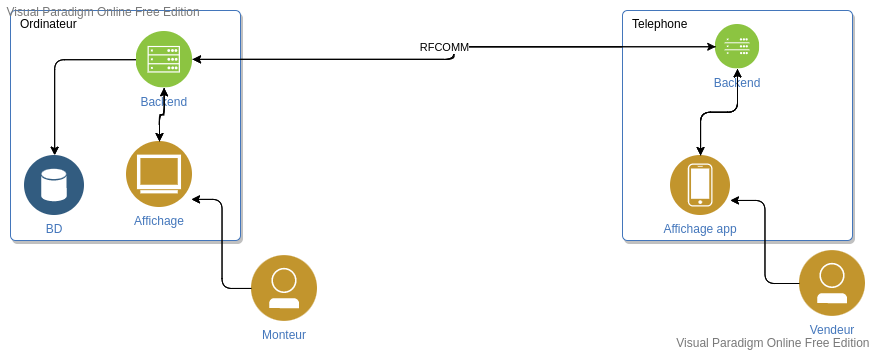
\includegraphics[scale=0.5]{images/architecture_ift592.png}



\subsection{Tentative d'utilisation du BLE}
Dans un premier temps, nous nous sommes orienté vers le bluetooth low energy car il semble correspondre plus à notre besoin principal. Le transfert de données très legere avec peu d'énergie. On a assez rapidement réussi à connecter les deux appareils mais impossbile de se connecter à un service défini par le protocole. Donc impossible de recupérer des données. La librairie de google implanté dans chrome (https://web.dev/bluetooth/).
On a également utilisé des applications de simulation de device en BLE sur le telephone pour tester, sans resultats. Encore à ce jour nous savons que c'est pas possible de communiquer avec ce protocole entre nos deux appareils mais nous n'avons pas d'explication théorique pour le justifier. On suppose que la relation maitre/esclave ne s'établie pas bien entre deux appreils destiné a etre dans la majorité des cas maitre. 

\subsection{Utilisation du bluetooth classique}
Après voir abandonné la piste du BLE. On s'est penché vers l'utilisation du bluetooth classique. Pour nous amener vers cette piste on inspecter le code d'applications d'envois de message OpenSource en bluetooth sur telephone (Bluetooth Chat). On a remarqué ce n'est pas le BLE qui est utilisé. À partir de ce moment on a commencé à essayer des libraires pour ce type de bluetooth sur l'application de bureau. Le premier problème rencontrer en nodejs est que toutes les librairies bluetooth comme (node-bluetooth, bluetooth-serial-port) utilisent node-gyp. C'est un command-line tool qui permet de compiler des modules natifs en nodejs. Malgrès de nombre heures de travail impossible de réussir à faire compiler ces librairies pour les essayer et savoir si elles marchent. Node-gyp est connu pour avoir ce genre de problème, il faut la bonne version de nodejs, npm et python pour que tout marche correctement. Ainsi que la bonne version de la librairy. Beaucoup de dépendance qui augmente la possiblité de problème. Ne sachant meme pas si ces librairies aller fonctionner on s'est tourner vers une autre approche du coté de l'ordinateur, c'est à dire faire fonctionner le bluetooth en dehors du code avec uniquement des lignes de commandes simples. C'est à ce moment là qu'on a découvert le protocle RFCOMM et réussi à faire notre premiere preuve de concept en ligne de command sur ligne et avec l'application de test sur Android : Serial Bluetooth.

Ouverture de la connexion sur linux, puis connexion du téléphone.

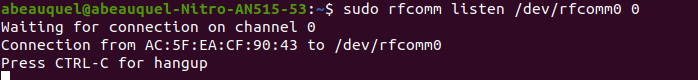
\includegraphics[scale=0.7]{images/rfcomm_connection_linux.png}


Envoie du message depuis le téléphone sur l'application Serial Bluetooth

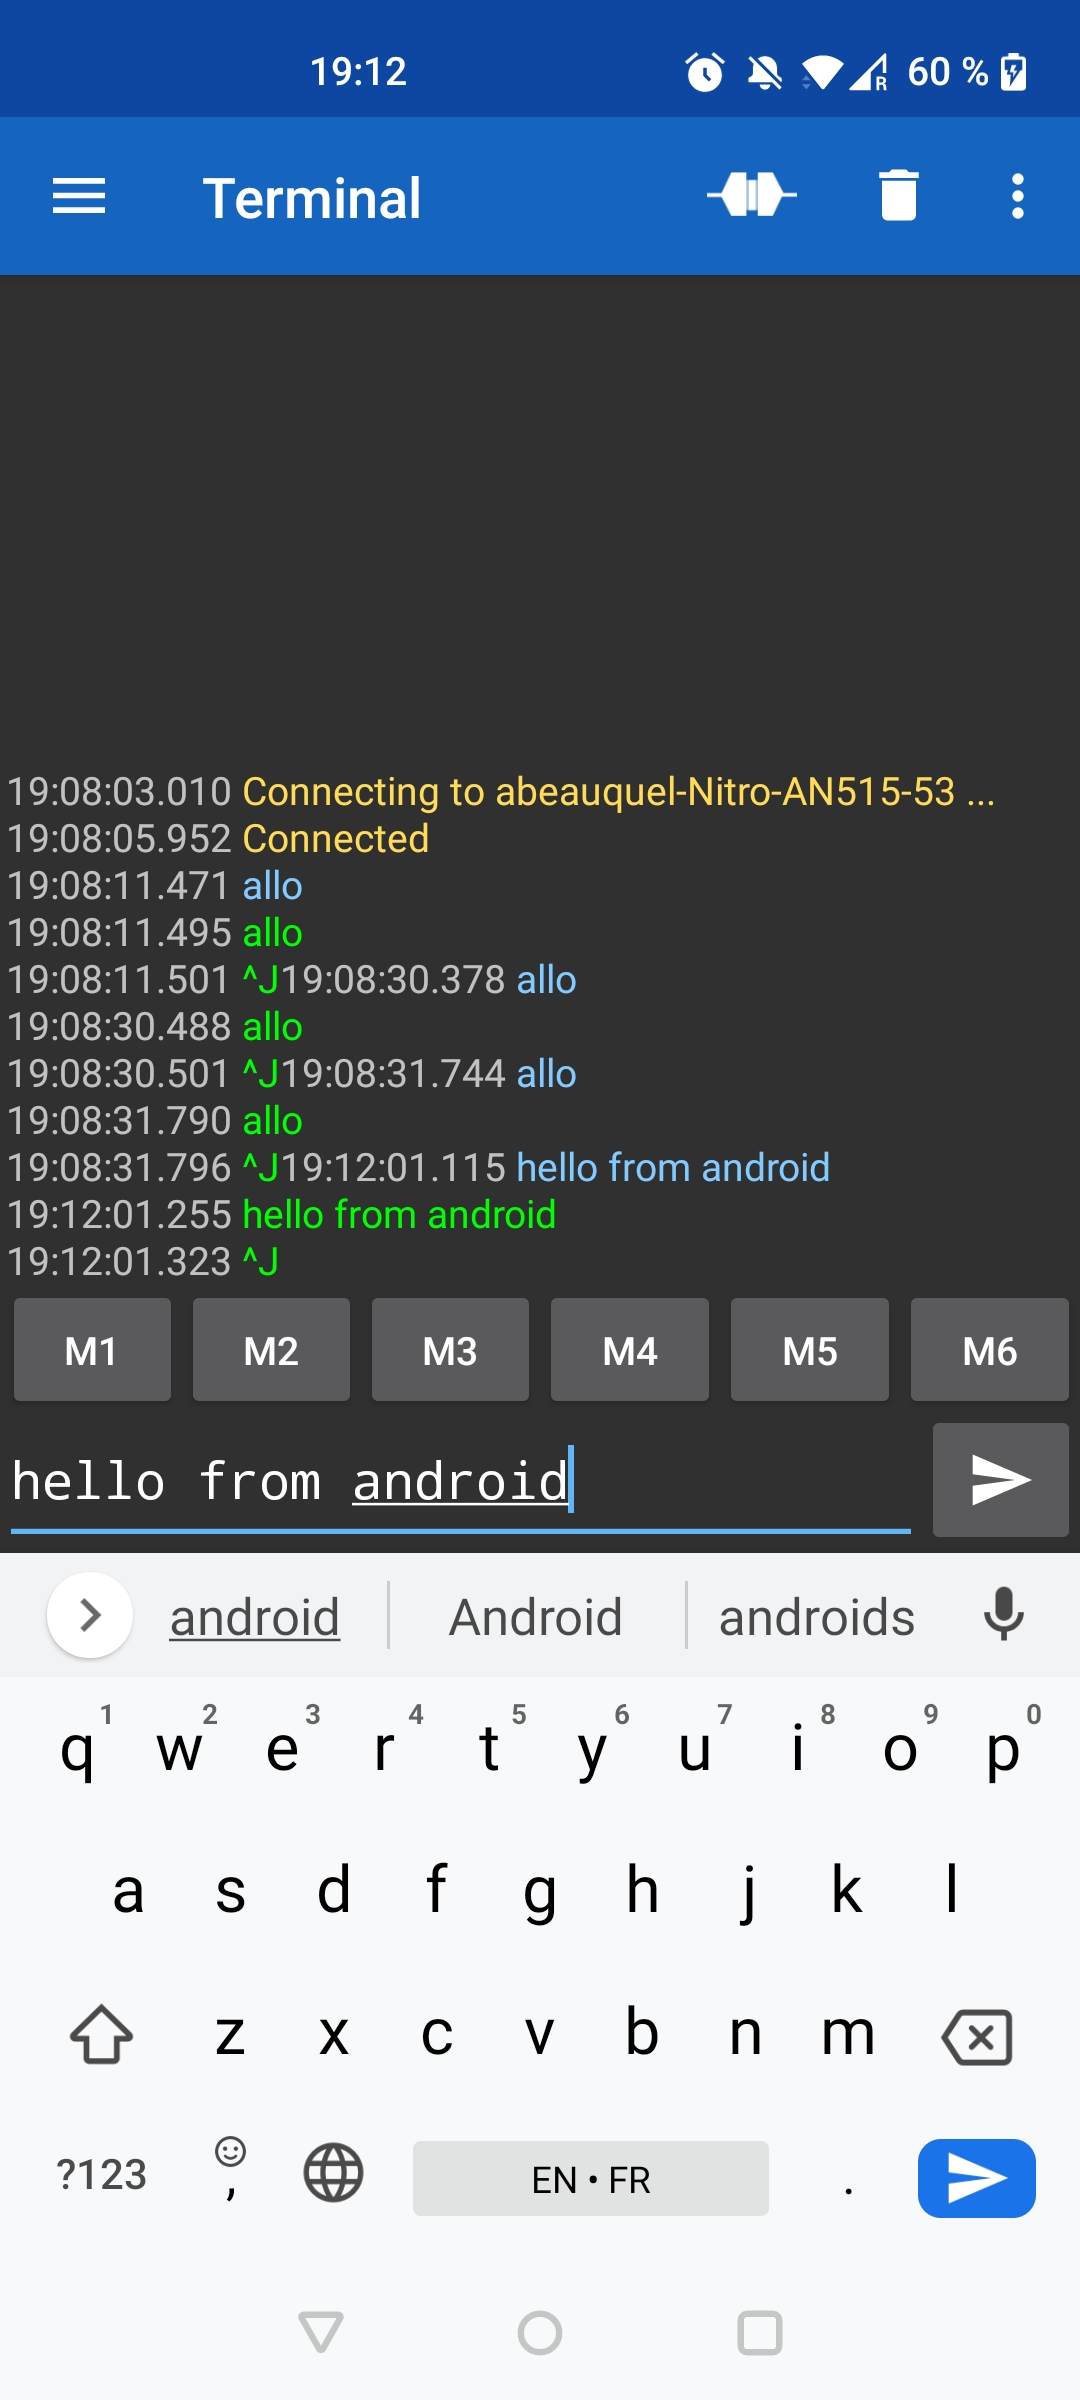
\includegraphics[scale=0.1]{images/rfcomm_telephone_message.jpg}

Lecture du message depuis linux

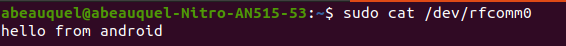
\includegraphics[scale=0.7]{images/rfcomm_linux_message.png}

Une fois cette preuve de concept réalisé on a décidé d'implanter notre propre librairie avec ces appels systèmes. 
\subsection{Fonctionnement du bluetooth dans le projet}
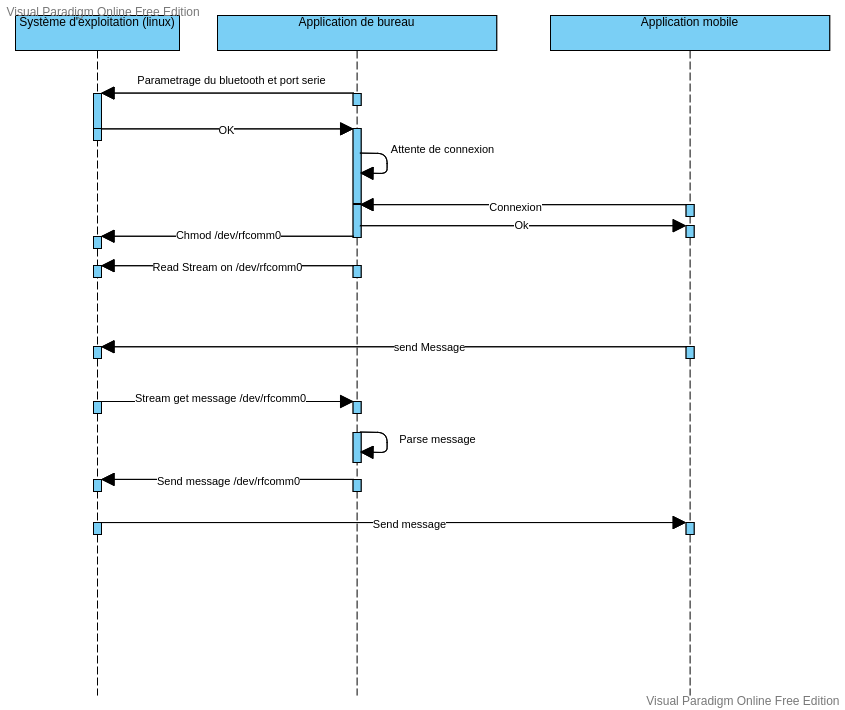
\includegraphics[scale=0.5]{images/sequence_bluetooth.png}

La fonction parseMessage sur l'application de bureau gère les messages suivant:
\begin{itemize}
\item création d'une commande
\item modification d'une commande
\item demande de la liste des commandes
\item demande d'un LS du dossier courant
\item demande d'un CD dans sous dossier
\item demande retour au dossier parent
\item demande recuperation d'une image
\end{itemize}
L'application de peut donc renvoyer au mobile les messages suivant :
\begin{itemize}
\item liste des commandes
\item LS du dossier courant
\item CD dans sous dossier
\item Retour au dossier parent
\item Image
\end{itemize}

\subsection{Resultat obtenue}
Ce qui marche et ne marche pas 

\subsection{Analyse des resultats}
abandon du crossplateforme


Les sections suivantes contiennent le corps du projet. Celui-ci est divisé en sections qui elles-mêmes sont divisées
en sous-sections.


Ces sections présentent :

\begin{itemize}
\item une introduction au sujet traité si cela est nécessaire;
\item les technologies utilisées avec justification;
\item la documentation technique (spécifications, architecture, conception);
\item la documentation pour l'utilisation (compilation, installation, interface, API, utilisation);
\item les tests effectuées et les résultats obtenus;
\item Une analyse des résultats si cela est pertinent.
\end{itemize}



\section{Conclusion}

La conclusion effectue un retour sur son travail. Expliquez les problèmes rencontrés lors de la réalisation de votre projet. Il est souhaitable de mentionner les perspectives de développements futurs.

\section{Annexes}

Ces sections sont optionnelles.  On met ici tout ce qui est trop lourd pour être intégré dans le texte.  On peut y mettre par exemple, des bouts de code ou d'algorithme qui sont trop long pour le texte. On peut y mettre le mandat original ainsi que les documents produits en cours de projets.


\section{Bibliographie}
\vspace{-0.75cm}
\renewcommand\refname{}

\bibliographystyle{plain-fr}
\bibliography{bibliographie}
\nocite{*}


\end{document}
